\documentclass[a4paper,12pt]{report}
\usepackage[utf8]{inputenc}
\usepackage{amsmath}
\usepackage{graphicx}
\usepackage{listings}
\usepackage{tikz}
\usepackage[T1]{fontenc}
\usepackage{color}
\usetikzlibrary{arrows,automata}
\definecolor{pythonred}{rgb}{0.6,0,0} % for strings
\definecolor{pythongreen}{rgb}{0.25,0.5,0.35} % comments
\definecolor{pythonpurple}{rgb}{0.5,0,0.35} % keywords
	\definecolor{pythondocblue}{rgb}{0.25,0.35,0.75} % javadoc
	\renewcommand{\thechapter}{}
	\renewcommand{\chaptername}{}
	\lstset{language=python,
	basicstyle=\ttfamily,
	keywordstyle=\color{pythonpurple}\bfseries,
	stringstyle=\color{pythonred},
	commentstyle=\color{pythongreen},
	morecomment=[s][\color{pythondocblue}]{/**}{*/},
	numbers=left,
	numberstyle=\tiny\color{black},
        stepnumber=2,
	numbersep=10pt,
	tabsize=4,
	showspaces=false,
	showstringspaces=false}

% Title Page

 \title{\bfseries\huge \textcolor{red}{\underline {EEP-702 Software Lab}} \\{\textcolor{blue}{Assignment1-Writing a Code to solve two problems}}}
\author{\bfseries\large\textcolor{black} {Harshit Kumar Gupta}\\ {\textcolor{black}{2013EET2369}}\\

\includegraphics[width=3cm,height=3.4cm]{./iit.png}\\\noindent Computer Technology\\
\noindent Department Of Electrical Engineering\\IIT DELHI}
% iit.png: 282x282 pixel, 72dpi, 9.95x9.95 cm, bb=0 0 282 282
\begin{document}
\maketitle
\tableofcontents


\chapter{\textcolor{blue}{\underline {PROBLEM STATEMENT}}}
\noindent 

         Write a program in C/C++/Java to solve following two problems:
	\begin{enumerate}
	\item To print matrix (M) elements in reverse spiral order i.e., starting from the centre element, print all the elements in spiral order until the first element M[0][0] is reached. Matrix M is of order n where n is odd.
        \item To match two strings containing wildcard characters '?' and '*' . '?' denotes no or exactly one character and '*' denotes no or many characters.
	\end{enumerate}

\begin{center}
\chapter{\textcolor{blue}{\underline {ABSTRACT}}}
\end{center}
\noindent The code has been entirely structured on C language. For the first preliminary code has been taken against the test cases for a 3*3 matrix, however further it was taken into a 
generalised form for the sake of robustness. Error handling has been tried so as the code works in case of a odd number ordered sqaure matrix, where the matrix is traversed right from
the center element to the final elememt that is the first ofcourse.
Second Code has been done through pointers and is well explained undr below.

\begin{center}
\chapter{\textcolor{blue}{\underline {INTRODUCTION}}}
\end{center}
\noindent \textbf Right from the starting when programming languages were developed, it was rather in the decade of 80s C language emerged which was much engraved with a powerful 
logic and soundness towards the logic and understanding.
Throughout my code has been entirely written on C. Matrix Operations are some of the most common logic applications in a C code. Furthermore the other code signifies using a Automata
set to check for the matching of two strings, where one of them contains a wild character.


\begin{center}
\chapter{\textcolor{blue}{\underline {SPECIFICATIONS AND ASSUMPTIONS}}}
\end{center}
\section*{Specifications}
\begin{enumerate}
\item gcc Compiler has been used to compile the code. 
\item gdb debugger may be used if some error is encountered.
\item Some places inspite of printf command puts has been used to display a string
\item If '*' is encountered it is treated as any number of characters or null.
\item If '?' is encountered it is treated as one character or null.


 \end{enumerate}
\section*{Assumptions}
\begin{enumerate}

\item User will be only allowed to put * and ? as special characters nothing else except alphabets.
\item The matrix would be an square Matrix
\item User will be providing a odd number ordered Matrix
\end{enumerate}
 
\begin{center}
\chapter{\textcolor{blue}{\underline {METHODOLOGY}}}
\end{center}
The methodology that is used for developing this project work is defined below:
\begin{enumerate} 
\item For the MATRIX TRAVERSAL CODE the idea was to go in an reverse spiral order.
\item Basically 4 'for' loops have been used which works as , the first loop prints the character towards the left from the center.
\item The second loop moves from left to right traversing the characters till upto the next column from the middle element so as to form a spiral.
\item The third and the fourth loop traverses for the remaining columns and rows respectively.
\item This is how we finally reach the end of the Traversal so as to reach the final element of the Matrix\\
\end{enumerate}

\section*{Second Problem}
\begin{enumerate}

\item In the Second Code for the String matching has to be done. 
\item As one of the Strings contain Wild Characters we have to implement the logic as per the specification. 
\item User will be providing a odd number ordered Matrix
\item Now the logic is that string is first of all matched as if through a naive approach, however when a * is countered the fuction is recursively called to match to the second character value.
\end{enumerate}


\begin{center}
\chapter{\textcolor{blue}{\underline {FLOWCHART}}}


 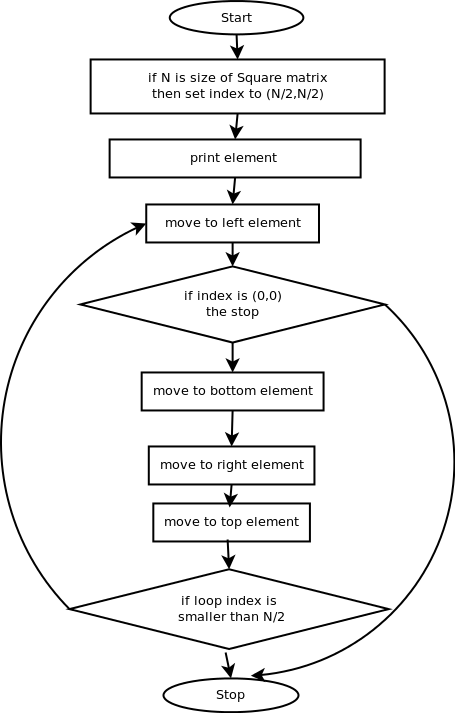
\includegraphics[width=15 cm,height=15 cm]{./flowchart1.png}
 % flowchart.png: 668x744 pixel, 72dpi, 23.57x26.25 cm, bb=0 0 668 744
\end{center}
\begin{center}
 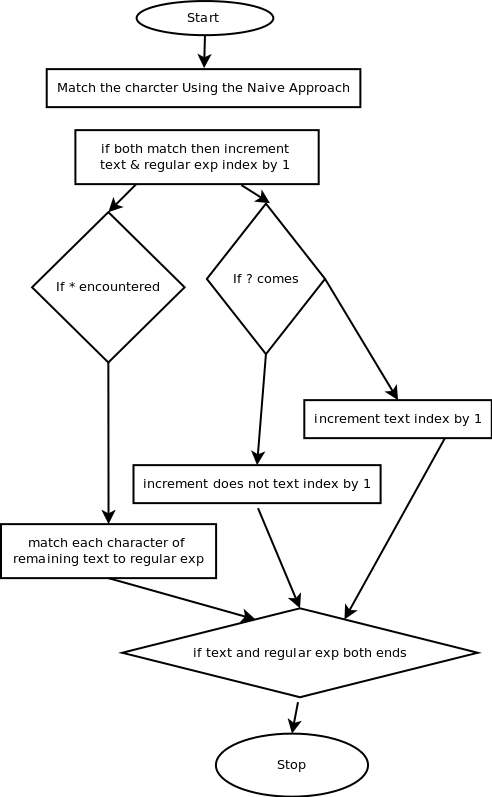
\includegraphics[width=15 cm,height=15 cm]{./flowchart2.png}
 % flowchart.png: 668x744 pixel, 72dpi, 23.57x26.25 cm, bb=0 0 668 744
\end{center}


\begin{center}
\chapter{\textcolor{blue}{\underline {OUTPUT}}}

 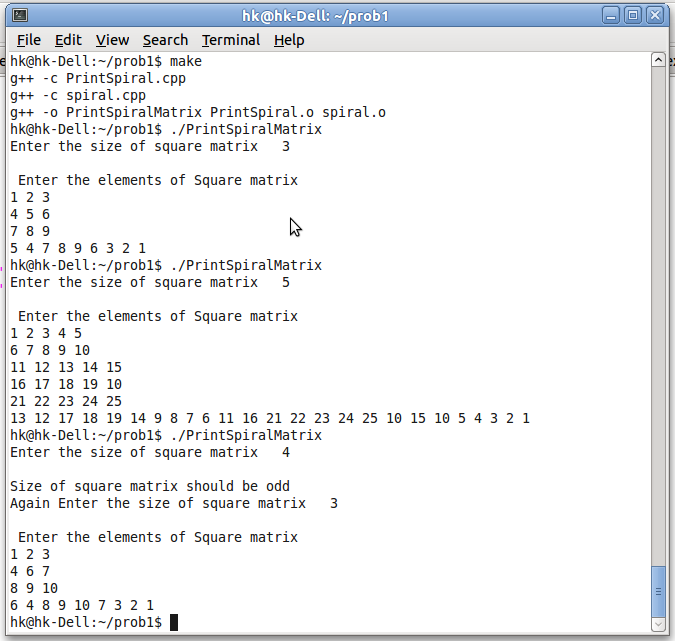
\includegraphics[width=13 cm,height=13 cm]{./output1.png}
 % flowchart.png: 668x744 pixel, 72dpi, 23.57x26.25 cm, bb=0 0 668 744

Output of Problem 1
\end{center}
\begin{center}
 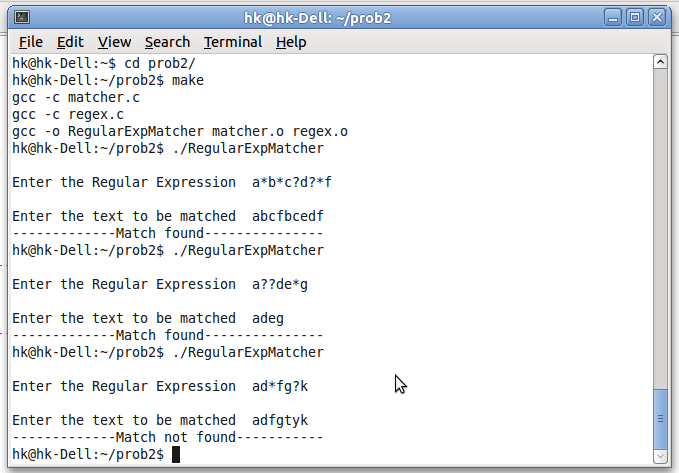
\includegraphics[width=13 cm,height=13 cm]{.//output2.png}
 % flowchart.png: 668x744 pixel, 72dpi, 23.57x26.25 cm, bb=0 0 668 744

Output of problem 2
\end{center}



\begin{center}
\chapter{\textcolor{blue}{\underline {RESULTS AND CONCLUSIONS}}}\end{center}

\noindent In both the cases the value output of the C and c++code is displayed on the user screen using the printf or cout command for the strings. In both the cases the output comes out to  be as expected and is verified for all the conditions.



\end{document}  
